    
    %%
    %% Sintel train final
    %%
    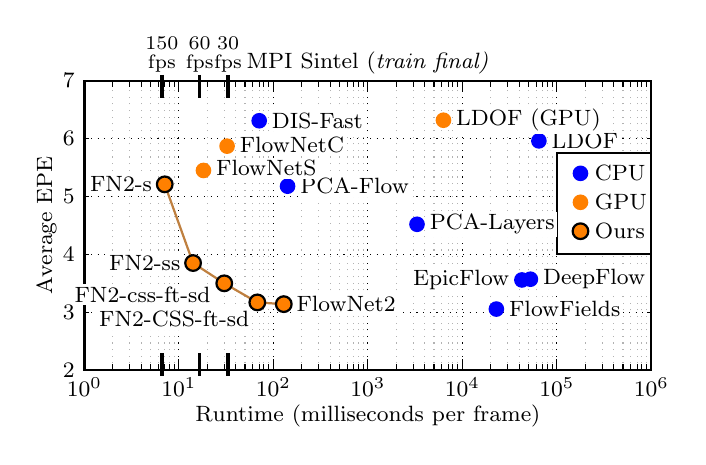
\begin{tikzpicture}[%
      font=\footnotesize,%
      xscale=1.2,yscale=1.75*.42,%
      cpunode/.style={fill=blue,circle,scale=.6},%
      gpunode/.style={fill=orange,circle,scale=.6},%
      ournode/.style={fill=orange,draw,thick,circle,scale=.6},%
      l/.style={fill=white,inner sep=1pt}%
    ]%
      %% Grid
      \draw[dotted] (0,0) grid (6,5);%
      %% X logarithm "grid"
      \foreach \logbase in {0,1,...,5} {%
        \foreach \log in {.3,.48,.6,.7,.78,.85,.9,.95} {%
          \draw[dotted,black!30] ({\logbase+\log},0) -- ++(0,5);%
        }%
      }%
      %% Frame
      \draw[thick] (0,0) -- ++(6,0) -- ++(0,5) -- ++(-6,0) -- cycle;%
      %% Title
      \node at (3,5.3) {MPI Sintel (\textit{train final)}};%
      %% Axes labels
      \node[rotate=90] at (-.4,2.5) {Average EPE};%
      \node at (3,-.8) {Runtime (milliseconds per frame)};%
      %% Y base ticks
      \foreach \y in {2,3,...,7} {%
        \node at (0,{\y-2}) [anchor=east] {$\y$};%
        \draw (0,{\y-2}) -- ++(.05,0);%
        \draw (6,{\y-2}) -- ++(-.05,0);%
      }%
      %% X base ticks
      \foreach \x in {0,1,...,6} {%
        \node at (\x,-.3) {$10^{\x}$};%
        \draw (\x,0) -- ++(0,.2);%
        \draw (\x,5) -- ++(0,-.2);%
      }%
      %% X logarithm ticks
      \foreach \logbase in {0,1,...,5} {%
        \foreach \log in {.3,.48,.6,.7,.78,.85,.9,.95} {%
          \draw ({\logbase+\log},0) -- ++(0,.1);%
          \draw ({\logbase+\log},5) -- ++(0,-.1);%
        }%
      }%
      %% Legend
      \draw[thick,fill=white] (5,2) rectangle ++(1,1.75);%
      \node[cpunode] at (5.25,3.4) {};%
      \node at (5.3,3.4) [anchor=west] {CPU};%
      \node[gpunode] at (5.25,2.9) {};%
      \node at (5.3,2.9) [anchor=west] {GPU};%
      \node[ournode] at (5.25,2.4) {};%
      \node at (5.3,2.4) [anchor=west] {Ours};%
      
      %% 150/60/30fps lines
      \draw[very thick] (0.82,5.1) -- ++(0,-0.4);
      \draw[very thick] (0.82,-.1) -- ++(0,0.4);
      \node at (0.82,5.65) {\scriptsize $150$};
      \node at (0.82,5.3) {\scriptsize fps};
      \draw[very thick] (1.22,5.1) -- ++(0,-0.4);
      \draw[very thick] (1.22,-.1) -- ++(0,0.4);
      \node at (1.22,5.65) {\scriptsize $60$};
      \node at (1.22,5.3) {\scriptsize fps};
      \draw[very thick] (1.52,5.1) -- ++(0,-0.4);
      \draw[very thick] (1.52,-.1) -- ++(0,0.4);
      \node at (1.52,5.65) {\scriptsize $30$};
      \node at (1.52,5.3) {\scriptsize fps};
      
      %% The Frontier Of Awesome
      \draw[brown,thick] (0.85,3.21)--(1.15,1.85)--(1.48,1.50)--(1.83,1.17)--(2.11,1.14);
      
      %% Points
      \node[cpunode] at (4.63,{3.558-2}) {};%
      \node[cpunode] at (4.72,{3.571-2}) {};%
      \node[cpunode] at (4.36,{3.055-2}) {};%
      \node[cpunode] at (4.81,{5.961-2}) {};%
      \node[gpunode] at (3.80,{6.318-2}) {};%
      \node[cpunode] at (2.15,{5.178-2}) {};%
      \node[cpunode] at (3.52,{4.520-2}) {};%
      \node[cpunode] at (1.85,{6.309-2}) {};%
      \node[gpunode] at (1.26,{5.45 -2}) {};%
      \node[gpunode] at (1.51,{5.87 -2}) {};%
      \node[ournode] at (0.85,{5.21 -2}) {};%
      \node[ournode] at (1.15,{3.85 -2}) {};%
      \node[ournode] at (1.48,{3.50 -2}) {};%
      \node[ournode] at (1.83,{3.17 -2}) {};%
      \node[ournode] at (2.11,{3.14 -2}) {};%
      \node[l]at({4.63-.1},{3.558-2})[anchor=east]{EpicFlow};%
      \node[l]at({4.72+.1},{3.571-2})[anchor=west]{DeepFlow};%
      \node[l]at({4.36+.1},{3.055-2})[anchor=west]{FlowFields};%
      \node[l]at({4.81+.1},{5.961-2})[anchor=west]{LDOF};%
      \node[l]at({3.80+.1},{6.318-2})[anchor=west]{LDOF (GPU)};%
      \node[l]at({2.15+.1},{5.178-2})[anchor=west]{PCA-Flow};%
      \node[l]at({3.52+.1},{4.520-2})[anchor=west]{PCA-Layers};%
      \node[l]at({1.85+.1},{6.309-2})[anchor=west]{DIS-Fast};%
      \node[l]at({1.26+.1},{5.45 -2+.04})[anchor=west]{FlowNetS};%
      \node[l]at({1.51+.1},{5.87 -2+.02})[anchor=west]{FlowNetC};%
      \node[l]at({0.85-.1},{5.21-2})[anchor=east]{FN2-s};%
      \node[l]at({1.15-.1},{3.85-2})[anchor=east]{FN2-ss};%
      \node[l]at({1.48-.11},{3.50-2.0})[anchor=north east]{FN2-css-ft-sd};%
      \node[l]at({1.83-.05},{3.17-2.1})[anchor=north east]{FN2-CSS-ft-sd};%
      \node[l]at({2.11+.1},{3.14-2})[anchor=west]{FlowNet2};%
      %\foreach \x/\y/\color/\name in {%
      %  3.63/3.558/blue/EpicFlow, % 42.6 s/frame
      %  3.72/3.571/blue/DeepFlow, % 51.94 s/frame
      %  3.36/3.055/blue/FlowFields, % 22.81 s/frame
      %  3.81/5.961/blue/LDOF, % 64.9 s/frame
      %  2.80/6.318/orange/LDOF, % 6.27 s/frame
      %  1.15/5.178/blue/PCA-Flow, % 0.14 s/frame
      %  2.52/4.520/blue/PCA-Layers, % 3.3 s/frame
      %  0.85/6.309/blue/DIS-Fast % 0.07 s/frame
      %} {%
      %  \node[fill=\color,circle,scale=.6] at (\x,\y) {};%
      %  \node at ({\x+.05},\y) [anchor=west] {\name};%
      %}%
    \end{tikzpicture}%
    
    %%
    %% KITTI 2012 train
    %%
    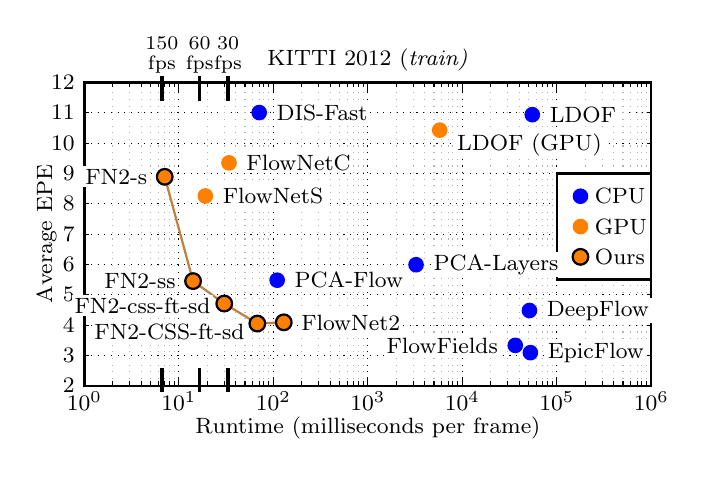
\begin{tikzpicture}[%
      font=\footnotesize,%
      xscale=1.2,yscale=1.75*.22,%
      cpunode/.style={fill=blue,circle,scale=.6},%
      gpunode/.style={fill=orange,circle,scale=.6},%
      ournode/.style={fill=orange,draw,thick,circle,scale=.6},%
      l/.style={fill=white,inner sep=1pt}%
    ]%
      %% Grid
      \draw[dotted] (0,0) grid (6,10);%
      %% X logarithm "grid"
      \foreach \logbase in {0,1,...,5} {%
        \foreach \log in {.3,.48,.6,.7,.78,.85,.9,.95} {%
          \draw[dotted,black!30] ({\logbase+\log},0) -- ++(0,10);%
        }%
      }%
      %% Frame
      \draw[thick] (0,0) -- ++(6,0) -- ++(0,10) -- ++(-6,0) -- cycle;%
      %% Title
      \node at (3,10.75) {KITTI 2012 (\textit{train)}};%
      %% Axes labels
      \node[rotate=90] at (-.4,5) {Average EPE};%
      \node at (3,-1.4) {Runtime (milliseconds per frame)};%
      %% Y base ticks
      \foreach \y in {2,3,...,12} {%
        \node at (0,{\y-2}) [anchor=east] {$\y$};%
        \draw (0,{\y-2}) -- ++(.05,0);%
        \draw (6,{\y-2}) -- ++(-.05,0);%
      }%
      %% X base ticks
      \foreach \x in {0,1,...,6} {%
        \node at (\x,-.5) {$10^{\x}$};%
        \draw (\x,0) -- ++(0,.3);%
        \draw (\x,10) -- ++(0,-.3);%
      }%
      %% X logarithm ticks
      \foreach \logbase in {0,1,...,5} {%
        \foreach \log in {.3,.48,.6,.7,.78,.85,.9,.95} {%
          \draw ({\logbase+\log},0) -- ++(0,.15);%
          \draw ({\logbase+\log},10) -- ++(0,-.15);%
        }%
      }%
      %% Legend
      \draw[thick,fill=white] (5,3.5) rectangle ++(1,3.5);%
      \node[cpunode] at (5.25,6.25) {};%
      \node at (5.3,6.25) [anchor=west] {CPU};%
      \node[gpunode] at (5.25,5.25) {};%
      \node at (5.3,5.25) [anchor=west] {GPU};%
      \node[ournode] at (5.25,4.25) {};%
      \node at (5.3,4.25) [anchor=west] {Ours};%
      
      %% 150/60/30fps lines
      \draw[very thick] (0.82,10.2) -- ++(0,-0.8);
      \draw[very thick] (0.82,-.2) -- ++(0,0.8);
      \node at (0.82,11.3) {\scriptsize $150$};
      \node at (0.82,10.6) {\scriptsize fps};
      \draw[very thick] (1.22,10.2) -- ++(0,-0.8);
      \draw[very thick] (1.22,-.2) -- ++(0,0.8);
      \node at (1.22,11.3) {\scriptsize $60$};
      \node at (1.22,10.6) {\scriptsize fps};
      \draw[very thick] (1.52,10.2) -- ++(0,-0.8);
      \draw[very thick] (1.52,-.2) -- ++(0,0.8);
      \node at (1.52,11.3) {\scriptsize $30$};
      \node at (1.52,10.6) {\scriptsize fps};
      
      %% The Frontier Of Awesome
      \draw[brown,thick] (0.85,6.89)--(1.15,3.45)--(1.48,2.71)--(1.83,2.05)--(2.11,2.09);
      
      %% Points
      \node[cpunode] at (4.72,{ 3.09-2}) {};%
      \node[cpunode] at (4.71,{ 4.48-2}) {};%
      \node[cpunode] at (4.56,{ 3.33-2}) {};%
      \node[cpunode] at (4.74,{10.94-2}) {};%
      \node[gpunode] at (3.76,{10.43-2}) {};%
      \node[cpunode] at (2.04,{ 5.48-2}) {};%
      \node[cpunode] at (3.51,{ 5.99-2}) {};%
      \node[cpunode] at (1.85,{11.01-2}) {};%
      \node[gpunode] at (1.28,{8.26 -2}) {};%
      \node[gpunode] at (1.53,{9.35 -2}) {};%
      \node[ournode] at (0.85,{8.89 -2}) {};%
      \node[ournode] at (1.15,{5.45 -2}) {};%
      \node[ournode] at (1.48,{4.71 -2}) {};%
      \node[ournode] at (1.83,{4.05 -2}) {};%
      \node[ournode] at (2.11,{4.09 -2}) {};%
      \node[l]at({4.72+.15},{ 3.09-2})[anchor=west]{EpicFlow};%
      \node[l]at({4.71+.15},{ 4.48-2})[anchor=west]{DeepFlow};%
      \node[l]at({4.56-.15},{ 3.33-2})[anchor=east]{FlowFields};%
      \node[l]at({4.74+.15},{10.94-2})[anchor=west]{LDOF};%
      \node[l]at({3.76+.15},{10.43-2})[anchor=north west]{LDOF (GPU)};%
      \node[l]at({2.04+.15},{ 5.48-2})[anchor=west]{PCA-Flow};%
      \node[l]at({3.51+.15},{ 5.99-2})[anchor=west]{PCA-Layers};%
      \node[l]at({1.85+.15},{11.01-2})[anchor=west]{DIS-Fast};%
      \node[l]at({1.28+.15},{8.26-2})[anchor=west]{FlowNetS};%
      \node[l]at({1.53+.15},{9.35-2})[anchor=west]{FlowNetC};%
      \node[l]at({0.85-.15},{8.89-2})[anchor=east]{FN2-s};%
      \node[l]at({1.15-.15},{5.45-2})[anchor=east]{FN2-ss};%
      \node[l]at({1.48-.11},{4.71-1.7})[anchor=north east]{FN2-css-ft-sd};%
      \node[l]at({1.83-.1},{4.05-1.9})[anchor=north east]{FN2-CSS-ft-sd};%
      \node[l]at({2.11+.15},{4.09-2})[anchor=west]{FlowNet2};%
      
      %\foreach \x/\y/\color/\name in {%
      %  2/6/blue/dummy %
      %} {%
      %  \node[fill=\color,circle,scale=.6] at (\x,{\y-4}) {};%
      %  \node at ({\x+.05},{\y-4}) [anchor=west] {\name};%
      %}%
    \end{tikzpicture}%
